\title{EC527 Lab 6: Open MP}
\author{John S. Burke}
\date{\today}

\documentclass[10pt,8.5in,11in]{article}

\usepackage{graphicx}
\usepackage{subcaption}
\usepackage[top=1.0in, bottom=1.0in, left=1.25in, right=1.25in]{geometry}

\begin{document}
	\maketitle
	
\section{Part One -- Hello World}

\paragraph{}
Quickly running test\_omp.c will show "Hello World" is always printed in order so that it makes sense.  This was done by using \texttt{\#pragma omp parallel for ordered} to control the loop.

\section{Part Two -- Parallel For}

\paragraph{}
For operations that are computationally intensive or bound by memory access, it can be clearly seen that once a certain amount of work has to be done there is obvious advantage to making use of Open MP.  However, when dealing with a situation where the overhead of Open MP is the bounding factor, it performs similarly to the baseline serial code.

\begin{figure}[h!]
\centering
\begin{subfigure}{.55\textwidth}
  \centering
  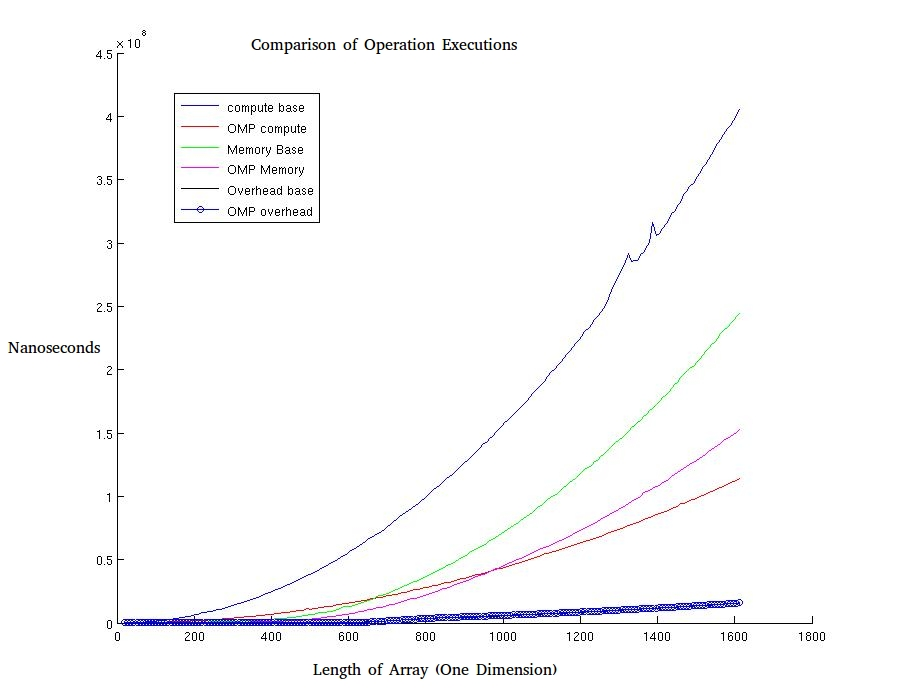
\includegraphics[width=\linewidth]{part2}
  \caption{Comparing Open MP with different loads}
\end{subfigure}%
\begin{subfigure}{.55\textwidth}
  \centering
  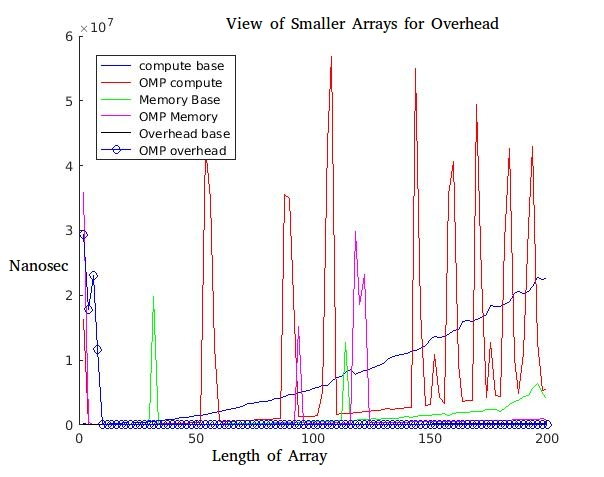
\includegraphics[width=\linewidth]{part2small}
  \caption{Zoomed in View of Left}
\end{subfigure}
\caption{Comparisons of Open MP with differing loads}
\end{figure}

\paragraph{}
Generally, an Open MP Parallel section is going to incur about 10 to 100 $\mu$s of overhead.  It's a bit easier to see this in certain situations in smaller arrays where parallelism isn't as immediately useful.  However, once out of this range for this kind of workload the parallelism has significant benefit.

\pagebreak
\section{Part Three -- Matrix Multiply}

	\subsection{Part A -- Initial Build}
	\paragraph{}	
	The Figure below shows the results of two versions of matrix multiply that differ in loop interchanges and the use of Open MP for a total of four implementations of the matrix multiply.
	
	\begin{figure}[h!]
	\centering
	\caption{Comparing Matrix Multiply in Given Code}
	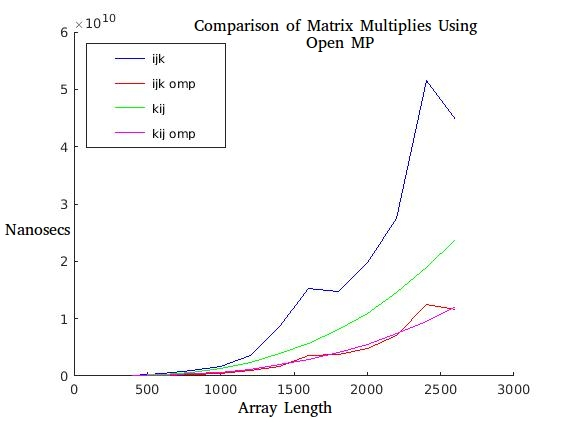
\includegraphics[scale=0.5]{part3a}
	\end{figure}
	
	\paragraph{}
	Much like was found in earlier assignments, the \texttt{kij} looping style performs better than the naturally conceived \texttt{ijk} style.  Furthermore, once the matrices become about 700 elements on a given side, the speed up from parallelizing is clear.  This is to be expected since matrix multiply is fairly compuationally intense, and the task can be easily split, making it a prime target for parallel implementations.
	
	\pagebreak
	\subsection{Part B -- Loop Indexes Shared}
	\paragraph{}
	Normally, loop indexes are private to a given element doing its own operations since where another thread may be reading from and calculating based off of should have no impact on other threads; they don't need to know where other threads are so long as the work is thoroughly parallel.
	
	\begin{figure}[h!]
	\centering
	\caption{Comparing Matrix Multiply with index variables shared}
	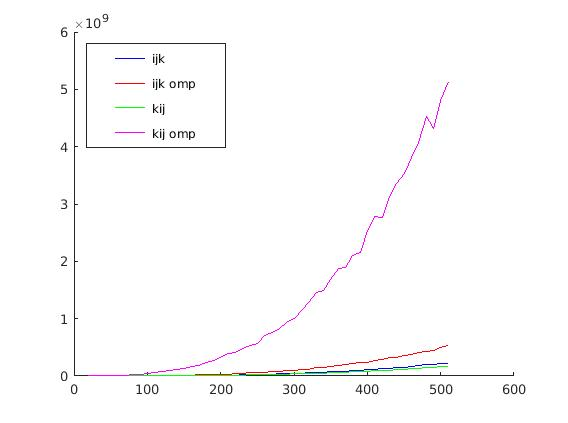
\includegraphics[scale=0.4]{part3b}
	\end{figure}
	
	\paragraph{}
	The most stark change is that \texttt{kij} in Open MP now does miserably when with it's total time inflating very quickly.  \texttt{ijk} maintains decent performance in this range, but still this causes the parallel versions to perform worse than the serial baselines.
	
	\subsection{Part C -- Moving the Parallel Sections}
	\paragraph{}	
	Normally for an operation like matrix multiply, it makes sense to parallelize every iterative element since each loop in it can be safely parallelized, but in this exercize we set the parallelization on only the inner loops with the following results.
	
	\begin{figure}[h!]
	\centering
	\begin{subfigure}{.5\textwidth}
  		\centering
  		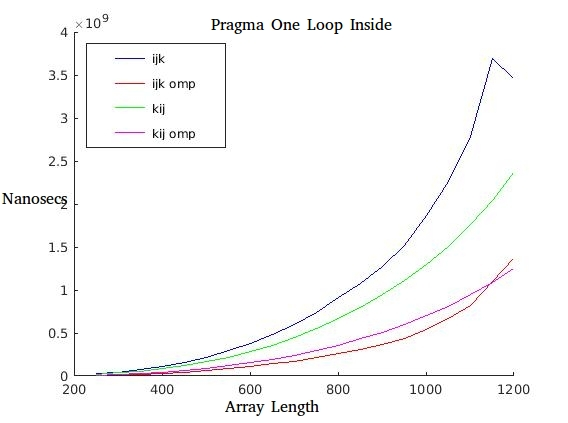
\includegraphics[width=\linewidth]{part3c_one}
  		\caption{Parallelize first inner loop}
	\end{subfigure}%
	\begin{subfigure}{.5\textwidth}
  		\centering
  		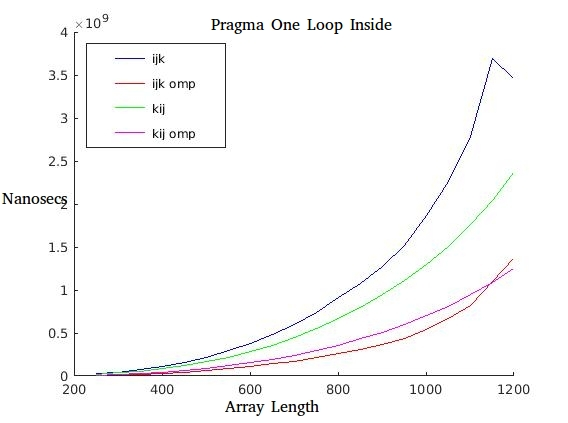
\includegraphics[width=\linewidth]{part3c_one}
  		\caption{Parallelize innermost loop}
	\end{subfigure}	
	\caption{Behavior when shifting what is parallelized}
	\end{figure}
	
	\paragraph{}
	add my info here
	
\pagebreak		
\section{Part Four -- Open MP with Real Programs}	

	\subsection{Part A -- SOR}
	
	\subsection{Part B -- Matrix Multiply}
	
\end{document}	
